\documentclass[20pt]{article}

\usepackage[us]{geometry}
\usepackage{titlesec}
\usepackage{amsmath}
\usepackage{amssymb}
\usepackage{times}
\usepackage{tipa}
\usepackage{covington}
\usepackage{tikz}
\usepackage{tikz-qtree}

\setlength\parindent{0pt}
\newcommand{\ipa}[1]{\textipa{#1}}
\newcommand{\broad}[1]{/\ipa{#1}/}
\newcommand{\narrow}[1]{[ \ipa{#1} ]}
\newcommand{\english}[1]{$<$#1$>$}
\newcommand{\sk}[0]{{\kern 0.05em}}
\newcommand{\mk}[0]{{\kern 0.1em}}
\newcommand{\smallcapi}[0]{\sk\textsci\sk}
\newcommand{\openo}[0]{\sk O}
\newcommand{\feature}[1]{\ensuremath{\left[ \text{#1} \right]}}
\newcommand{\treeScale}[0]{1}
\newcommand{\rolesOne}[0]{$<$$\theta$$>$}
\newcommand{\rolesTwo}[0]{$<$$\theta$,$\theta$$>$}
\newcommand{\rolesThree}[0]{$<$$\theta$,$\theta$,$\theta$$>$}

\titlespacing*{\section}{0pt}{0.7\baselineskip}{0.7\baselineskip}
\titleformat*{\section}{\large\bfseries}

\begin{document}

\Large\textbf{Problem Set 4} \\
\normalsize
Alice McKean \\
\today

\section{Phrase Structure Trees}

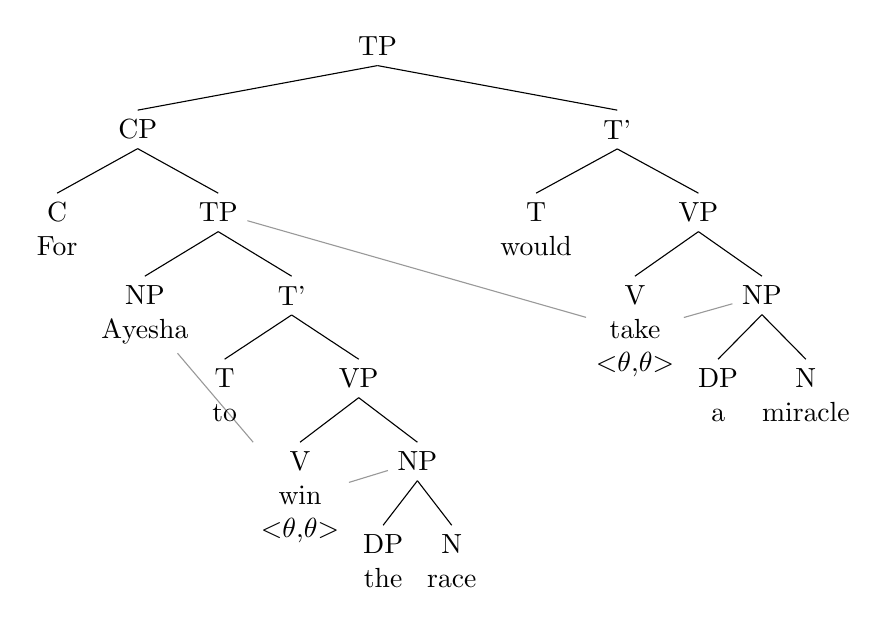
\begin{tikzpicture}[scale=\treeScale, transform shape]
  \tikzset{every tree node/.style={align=center,anchor=north}}
  \Tree [.TP [.CP C\\For
                  [.\node(s2e1){TP}; \node(s1e1){NP\\Ayesha};
                       [.T' T\\to
                            [.VP \node(s1){V\\win\\\rolesTwo};
                                 [.\node(s1e2){NP};
                                      DP\\the
                                      N\\race
                                 ]
                            ]
                       ]
                  ]
             ]
             [.T' T\\would
                  [.VP \node(s2){V\\take\\\rolesTwo};
                       [.\node(s2e2){NP}; DP\\a
                            N\\miracle
                       ]
                  ]
             ]
        ]
        \draw[opacity=0.4] (s1) -- (s1e2);
        \draw[opacity=0.4] (s1) -- (s1e1);
        \draw[opacity=0.4] (s2) -- (s2e1);
        \draw[opacity=0.4] (s2) -- (s2e2);
\end{tikzpicture}


\begin{tikzpicture}[scale=\treeScale, transform shape]
  \tikzset{every tree node/.style={align=center,anchor=north}}
  \Tree [.TP \node(s1e1){NP\\Denny};
             [.T' T\\\feature{PAST}
                  [.VP \node(s1){V\\decide\\\rolesTwo};
                       [.\node(s1e2){TP}; \node(s2e1){NP\\\feature{PRO}};
                            [.T' T\\to
                                 [.VP \node(s2){V\\write\\\rolesTwo};
                                      [.\node(s2e2){NP}; DP\\a
                                           [.N' AP\\new
                                                N\\novel
                                           ]
                                      ]
                                 ] 
                            ]
                       ]
                  ]
             ]
        ]
        \draw[opacity=0.4] (s1) -- (s1e1);
        \draw[opacity=0.4] (s1) -- (s1e2);
        \draw[opacity=0.4] (s2) -- (s2e1);
        \draw[opacity=0.4] (s2) -- (s2e2);
\end{tikzpicture}

\begin{tikzpicture}[scale=\treeScale, transform shape]
  \tikzset{every tree node/.style={align=center,anchor=north}}
  \Tree [.TP NP\\{It}
             [.T T\\\feature{PRES}
                 [.VP \node(s1){V\\seem\\\rolesOne};
                      [.CP C\\that
                           [.\node(s1e1){TP}; [.\node(s2e1){NP}; DP\\that
                                     N\\puppy
                                ]
                                [.T' T\\has
                                     [.VP \node(s2){V\\become\\\rolesTwo};
                                          [.\node(s2e2){AP}; DegP\\rather
                                               [.AP A\\fond
                                                    [.PP P\\of
                                                         NP\\you
                                                    ]
                                               ]
                                          ]
                                     ]
                                ]
                           ]
                      ]
                 ]
             ]
        ]
        \draw[opacity=0.4] (s1) -- (s1e1);
        \draw[opacity=0.4] (s2) -- (s2e1);
        \draw[opacity=0.4] (s2) -- (s2e2);
\end{tikzpicture}

\begin{tikzpicture}[scale=\treeScale, transform shape]
  \tikzset{every tree node/.style={align=center,anchor=north}}
  \Tree [.TP [.\node(s1e1){NP}; DP\\The
                  N\\police
             ]
             [.T' T\\\feature{PRES}
                  [.VP \node(s1){V\\believe\\\rolesTwo};
                       [.\node(s1e2){TP}; \node(s2e1){NP\\Norbert};
                            [.T' T\\to 
                                 [.VP \node(s2){V\\have\\\rolesTwo};
                                      [.\node(s2e2){TP}; \node(s3e1){NP\\\feature{PRO}};
                                           [.T' T\\\feature{PAST}
                                                [.VP \node(s3){V\\commit\\\rolesTwo};
                                                     [.\node(s3e2){NP}; DP\\the
                                                          N\\crime
                                                     ]
                                                ]
                                           ]
                                      ]
                                 ]
                            ]
                       ]
                  ]
             ]
        ]
        \draw[opacity=0.4] (s1) -- (s1e1);
        \draw[opacity=0.4] (s1) -- (s1e2);
        \draw[opacity=0.4] (s2) -- (s2e1);
        \draw[opacity=0.4] (s2) -- (s2e2);
        \draw[opacity=0.4] (s3) -- (s3e1);
        \draw[opacity=0.4] (s3) -- (s3e2);
\end{tikzpicture}

\begin{tikzpicture}[scale=\treeScale, transform shape]
  \tikzset{every tree node/.style={align=center,anchor=north}}
  \Tree [.TP [.\node(s1e1){NP};
                  DP\\The
                  N\\students
             ]
             [.T' T\\\feature{PAST}
                  [.VP \node(s1){V\\learn\\\rolesTwo};
                       [.CP C\\that  
                            [.\node(s1e2){TP}; [.PP P\\on
                                      NP\\Friday
                                 ]
                                 [.TP \node(s2e1){NP\\they};
                                      [.T' T\\will
                                           [.VP [.VP \node(s2){V\\have\\\rolesTwo};
                                                     [.\node(s2e2){NP}; DP\\a
                                                          N\\quiz
                                                     ]
                                                ]
                                                [.PP P\\in
                                                     NP\\class
                                                ]
                                           ]
                                      ]
                                 ]
                            ]
                       ]
                  ]
             ]
        ]
        \draw[opacity=0.4] (s1) -- (s1e1);
        \draw[opacity=0.4] (s1) -- (s1e2);
        \draw[opacity=0.4] (s2) -- (s2e1);
        \draw[opacity=0.4] (s2) -- (s2e2);
\end{tikzpicture}

\section{Clauses}

\begin{tabular}{l|l|l}
  Clause & Subject & Object \\
  \hline
  Sentence 1 & For Ayesha to win the race & a miracle \\ 
  Ayesha to win the race & Ayesha & the race \\
  & & \\
  Sentence 2 & Denny & to write a new novel \\
  \feature{PRO} to write a new novel & \feature{PRO} & a new novel \\
  & & \\
  Sentence 3 & It & that that puppy has become rather fond of you \\
  that puppy has become rather fond of you & that puppy & rather fond of you \\
  & & \\
  Sentence 4 & The police & Norbert to have committed the crime \\
  Norbert to have committed the crime & Norbert & committed the crime \\
  \feature{PRO} committed the crime & \feature{PRO} & the crime \\
  & & \\
  Sentence 5 & The students & that on Friday they will have a quiz in class \\
  On friday they will have a quiz in class & on Friday & $\emptyset$ \\
  they will have a quiz in class & They & a quiz \\
\end{tabular}

\section{Theta Roles}
Please see the trees.

\end{document}

